\documentclass[dvipdfmx]{jsarticle}


\usepackage{tcolorbox}
\usepackage{color}
\usepackage{listings, plistings}

%% ノート/latexメモ
%% http://pepper.is.sci.toho-u.ac.jp/pepper/index.php?%A5%CE%A1%BC%A5%C8%2Flatex%A5%E1%A5%E2

%% JavaScriptの設定
%% https://e8l.hatenablog.com/entry/2015/11/29/232800
\lstdefinelanguage{javascript}{
  morekeywords = [1]{ %keywords
    await, break, case, catch, class, const, continue, debugger, default, delete, 
    do, else, enum, export, extends, finally, for, function, function*, if, implements, import, in, 
    instanceof, interface, let, new, package, private, protected, public, return, static, super,
    switch, this, throw, try, typeof, var, void, while, with, yield, yield*
  },
  morekeywords = [2]{ %literal
    false, Infinity, NaN, null, true, undefined
  },
  morekeywords = [3] { %Classes
    Array, ArrayBuffer, Boolean, DataView, Date, Error, EvalError, Float32Array, Float64Array,
    Function, Generator, GeneratorFunction, Int16Array, Int32Array, Int8Array, InternalError,
    JSON, Map, Math, Number, Object, Promise, Proxy, RangeError, ReferenceError, Reflect,
    RegExp, Set, String, Symbol, SyntaxError, TypeError, URIError, Uint16Array, Uint32Array,
    Uint8Array, Uint8ClampedArray, WeakMap, WeakSet
  },
  morecomment = [l]{//},
  morecomment = [s]{/*}{*/},
  morestring = [b]{"},
  morestring = [b]{'},
  alsodigit = {-},
  sensitive = true
}

%% 修正時刻: Tue 2022/03/15 10:04:41


% Java
\lstset{% 
  frame=single,
  backgroundcolor={\color[gray]{.9}},
  stringstyle={\ttfamily \color[rgb]{0,0,1}},
  commentstyle={\itshape \color[cmyk]{1,0,1,0}},
  identifierstyle={\ttfamily}, 
  keywordstyle={\ttfamily \color[cmyk]{0,1,0,0}},
  basicstyle={\ttfamily},
  breaklines=true,
  xleftmargin=0zw,
  xrightmargin=0zw,
  framerule=.2pt,
  columns=[l]{fullflexible},
  numbers=left,
  stepnumber=1,
  numberstyle={\scriptsize},
  numbersep=1em,
  language={Java},
  lineskip=-0.5zw,
  morecomment={[s][{\color[cmyk]{1,0,0,0}}]{/**}{*/}},
  keepspaces=true,         % 空白の連続をそのままで
  showstringspaces=false,  % 空白字をOFF
}
%\usepackage[dvipdfmx]{graphicx}
\usepackage{url}
\usepackage[dvipdfmx]{hyperref}
\usepackage{amsmath, amssymb}
\usepackage{itembkbx}
\usepackage{eclbkbox}	% required for `\breakbox' (yatex added)
\usepackage{enumerate}
\usepackage[default]{cantarell}
\usepackage[T1]{fontenc}
\fboxrule=0.5pt
\parindent=1em
\definecolor{mygrey}{rgb}{0.97, 0.97, 0.97}

\makeatletter
\def\verbatim@font{\normalfont
\let\do\do@noligs
\verbatim@nolig@list}
\makeatother

\begin{document}

%\anaumeと入力すると穴埋め解答欄が作れるようにしてる。\anaumesmallで小さめの穴埋めになる。
\newcounter{mycounter} % カウンターを作る
\setcounter{mycounter}{0} % カウンターを初期化
\newcommand{\anaume}[1][]{\refstepcounter{mycounter}{#1}{\boxed{\phantom{aa}\textnormal{\themycounter}\phantom{aa}}}} %穴埋め問題の空欄作ってる。
\newcommand{\anaumesmall}[1][]{\refstepcounter{mycounter}{#1}{\boxed{\tiny{\phantom{a}\themycounter \phantom{a}}}}}%小さい版作ってる。色々改造できる。

%% 修正時刻: Tue 2022/03/15 10:04:411


\section{XAMPPのダウンロードとインストール}

\subsection{ダウンロード}

google などで、``xampp''で検索。

\vspace{3mm}
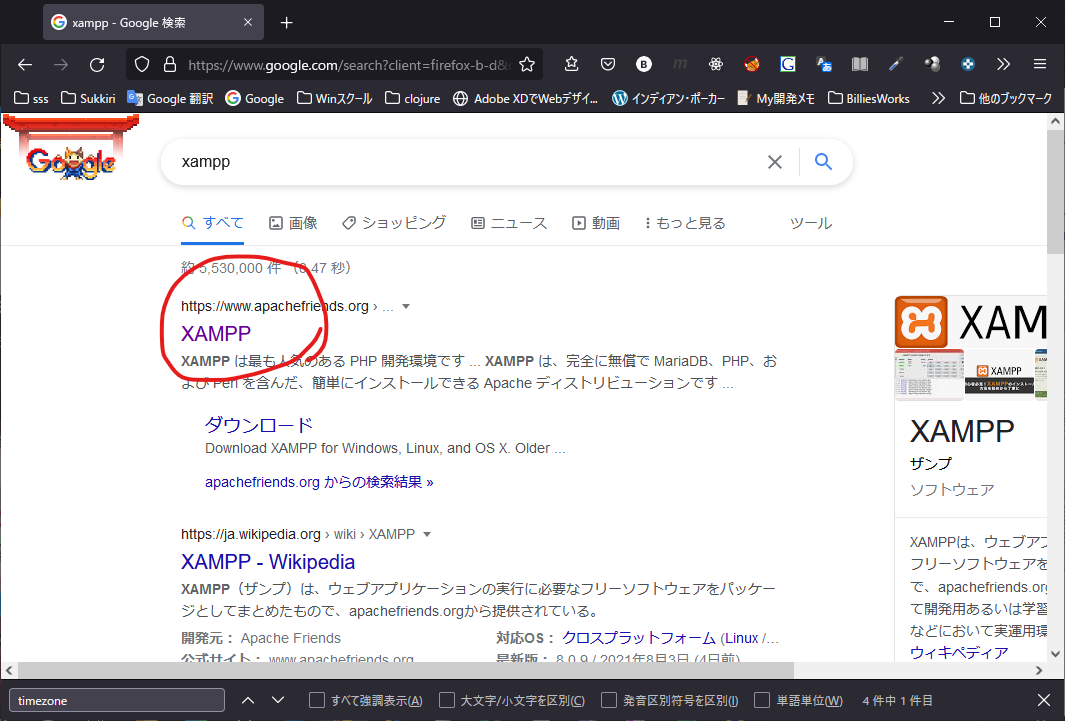
\includegraphics[width=13cm]{../01-download/01-xampp.png}
\vspace{3mm}

XAMPP のページが開くので、''Windows版'' をダウンロードする。

\vspace{3mm}
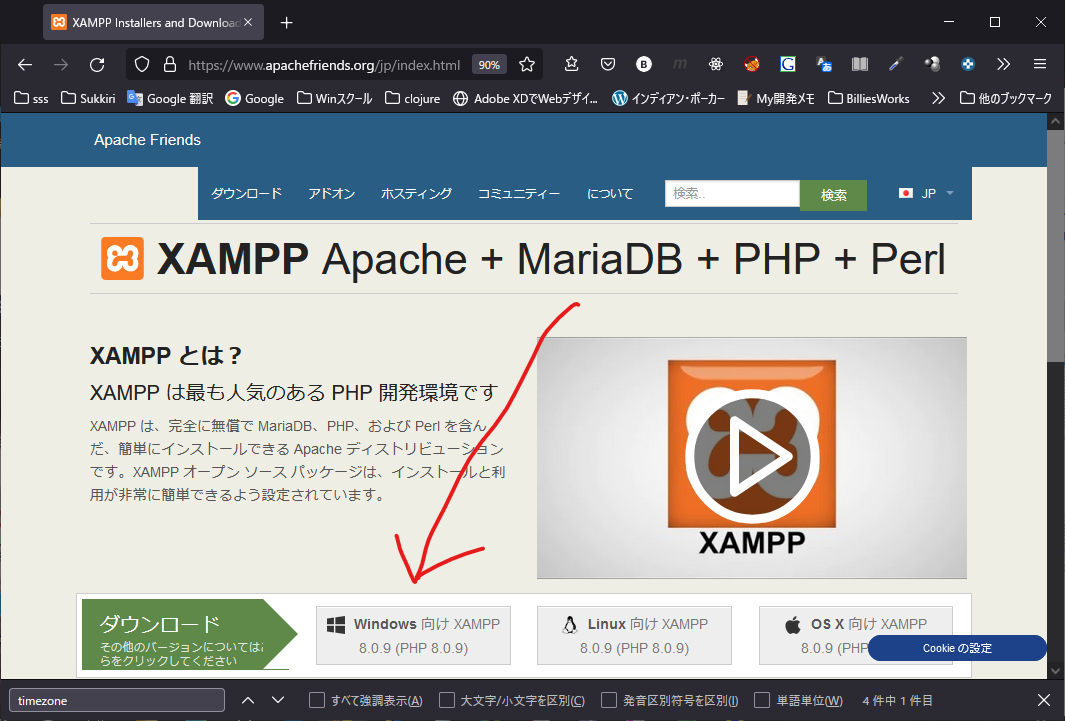
\includegraphics[width=13cm]{../01-download/02-xampp-download.png}
\vspace{3mm}

ファイルを保存する。``ダウンロード''フォルダに保存される。

\vspace{3mm}
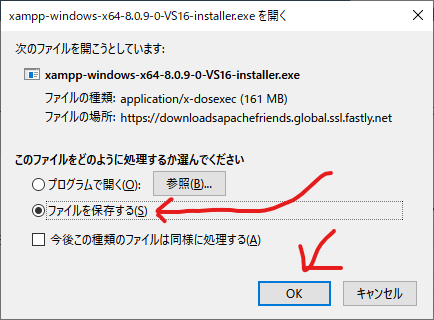
\includegraphics[width=10cm]{../01-download/03-xampp.png}
\vspace{3mm}

\subsection{インストール}

``ダウンロード'' フォルダの ``\textsf{xampp-windows-x64-8.0.9-0-VS16-install.exe}''
をダブルクリックしてインストールを実行する。

○○が Windows の変更を許可しますか? みたいなことが表示されたら、``はい'' を選択する。

次に英語で ''Warning'' が表示される。

\vspace{3mm}
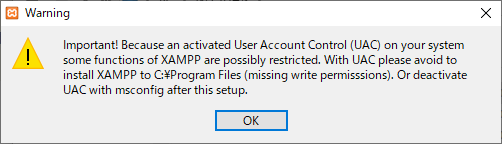
\includegraphics{../02-install/01-install.png}
\vspace{3mm}

Google翻訳
\begin{tcolorbox}
 重要! システムでアクティブ化されたユーザーアカウント制御(UAC)が原因で、XAMPPの一部の機能が制限されている可能性があります。 \\
 UACでは、XAMPPをC:\yen Program Filesにインストールしないでください(書き込み権限がありません)。 \\
 または、この設定後にmsconfigを使用してUACを非アクティブ化します。
\end{tcolorbox}

C:\yen Program Files にはインストールしないから、大丈夫。

次は、コンポーネントの選択画面である。

既定値では、すべてのコンポーネントが選択されているが、``FileZilla'' と ``Merucry'' と
``Tomcat'' は いらない。
インストールしても、使うことはまずない。

\vspace{3mm}
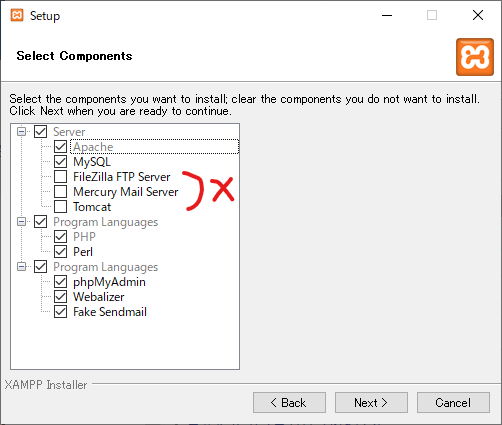
\includegraphics{../02-install/02-check.png}
\vspace{3mm}

インストール先の確認画面である。

\vspace{3mm}
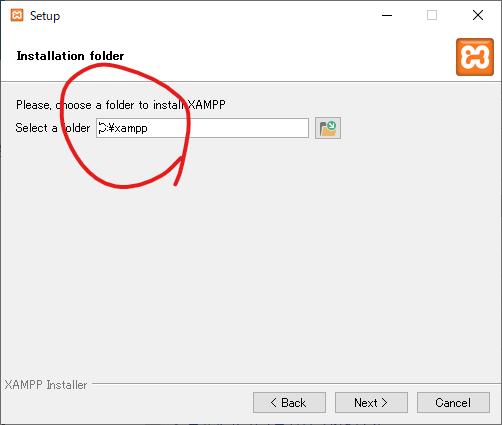
\includegraphics[width=9cm]{../02-install/03-folder.png}
\vspace{3mm}

\textsf{C:\yen XAMPP} にインストールされる。(覚えておく)

次は、\textsf{XAMPP Control Panel} ではどの言語を使うかを選択できる。
が、日本語はない。

\vspace{3mm}
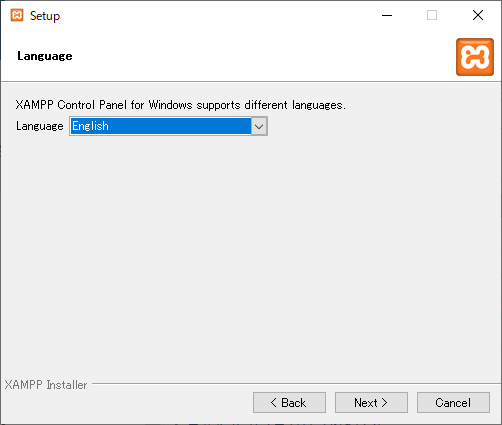
\includegraphics[width=10cm]{../02-install/04-english.png}
\vspace{3mm}

次の画面では、チェックをはずすが、これはチェックがはいったままでも
かまわない。
Bitnami for XAMPP についての情報へのリンクをつくるかどうかを
尋ねているだけである。

\vspace{3mm}
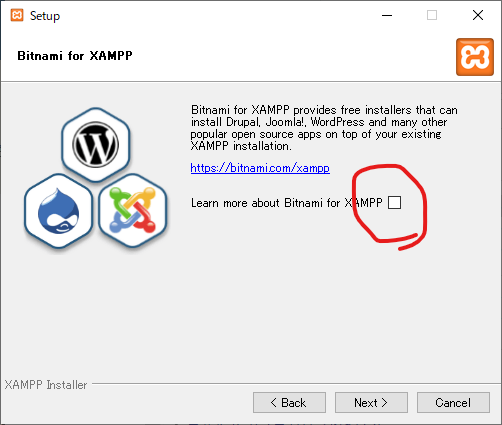
\includegraphics[width=10cm]{../02-install/05-no.png}
\vspace{3mm}

さて、これでインストールが実行される。しばらくかかる。

\subsection{インストール後のメニューの設定と起動}

インストールが終了すると、スタートメニューに XAMPP のメニューができている。

\textsf{XAMPP Control Panel} の項目を右クリックして、''スタートにピン留めする'' を
クリックして、スタートパネルから呼び出せるようにしておく。

\vspace{3mm}
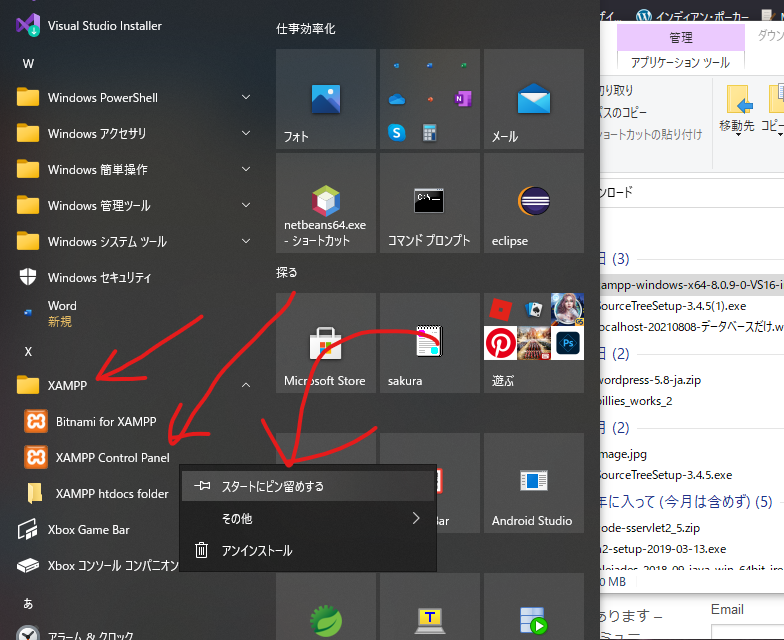
\includegraphics[width=13cm]{../02-install/06-start-panel.png}
\vspace{3mm}

\newpage
インストール直後の状態では、
XAMPPコントロールパネルを起動するときは、``管理者として実行'' をする必要がある。
右クリックして、``その他'' --- ``管理者として実行'' を選択する。


\vspace{3mm}
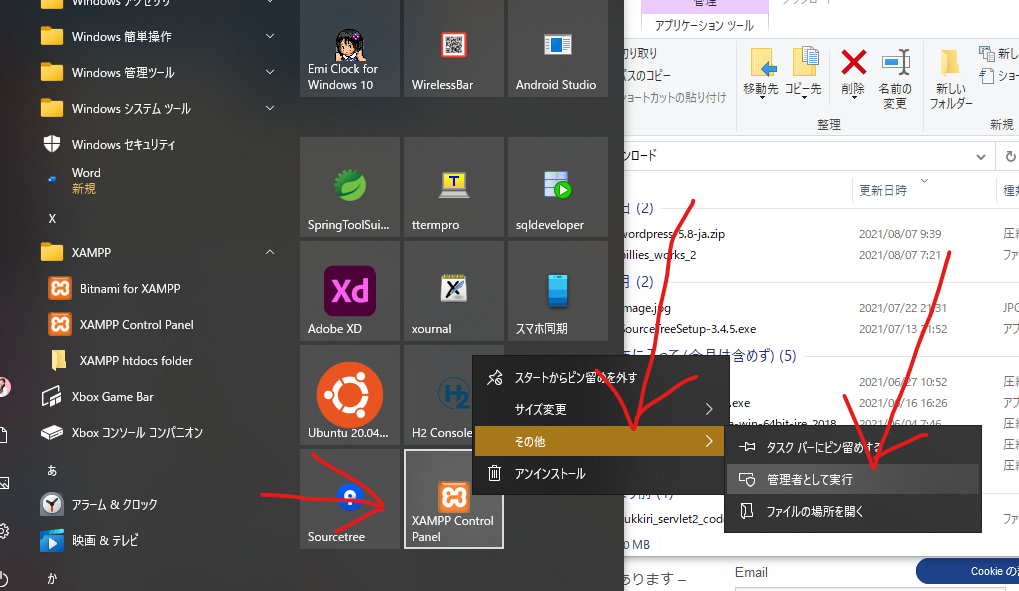
\includegraphics[width=14cm]{../02-install/07-kanrisya.png}
\vspace{3mm}

\subsection{管理者ユーザーで実行できるようにする}

右クリックしなくても、XAMPPコントロールパネルを
管理者ユーザーで起動できるようにする。

\textsf{C:\yen xampp} フォルダを開き、
``xampp-control.exe'' を右クリックして、
``プロパティ''を選択する。

\vspace{3mm}
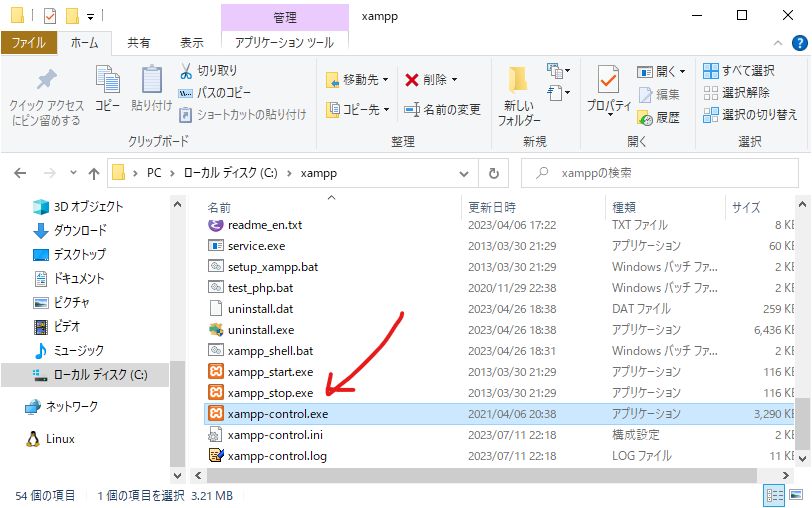
\includegraphics[width=10cm]{../02-install/20-xampp-ctrl-01.png}
\vspace{3mm}

\vspace{3mm}
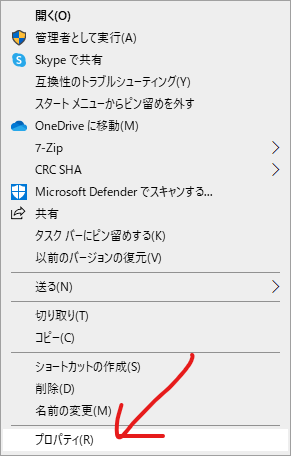
\includegraphics[width=4cm]{../02-install/21-xampp-ctrl-02.png}
\vspace{3mm}

``xampp-control.exeのプロパティ''のダイアログが開くので、
``互換性''タブを選択する。

\vspace{3mm}
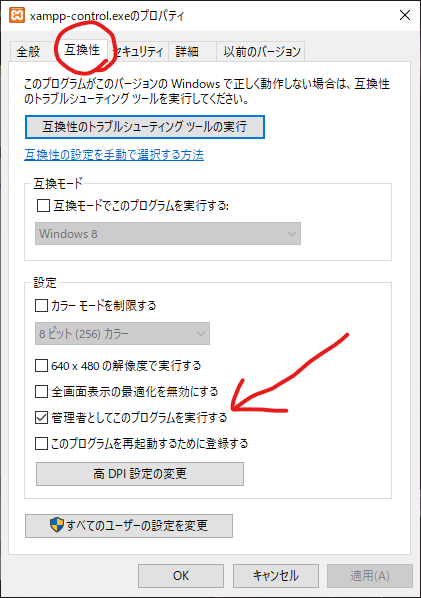
\includegraphics[width=6cm]{../02-install/22-xampp-ctrl-03.png}
\vspace{3mm}

開いた ``互換性''タブで、
`` 管理者としてこのプログラムを実行する''にチェックを入れて
``OK''とする。







\end{document}

%% 修正時刻: Sat May  2 15:10:04 2020


%% 修正時刻: Thu 2023/09/28 09:55:221
